\section{Notations}
\label{sec:reconstruction}
  
    % Limitation des approches de reconstruction de CFG à partir des fichiers
    % sources et nécessité du fichier exécutable pour la reconstruction de CFG.

    Soit $\mathcal{I}$ un ensemble fini d'instructions.
    Soit $\mathcal{L}$ un ensemble fini totalement ordonné d'étiquettes.
    Un programme $P$ est un sous-ensemble fini de $\mathcal{L} \times \mathcal{I}$ tel que
    $\forall (l,i) \in P,\quad (l,i') \in P \leftrightarrow i = i'$.
    On note $\mathcal{V}$ l'ensemble des variables de $P$.     
    Si l'on considère le programme de la figure~\ref{fig:dump}, $\mathcal{I}$
    est l'ensemble des instructions de l'ISA PowerPC 32 bits,
    $\mathcal{L}$ est l'ensemble des adresses mémoires alignées sur des
    frontières de 4 octets de la plage $[3000, 3034]$ et $\mathcal{V}$ est
    l'ensemble des registres utilisés explicitement ou implicitement (ici :
    $\{r1, r3, r8, r9, r10, lr, ctr\}$).

%    \begin{figure}[ht]
%      \centering
%      %\begin{subfigure}[t]{.20\textwidth}
%        \centering
%        \includegraphics[scale=.4]{img/dump.eps}
%        \captionsetup{justification=centering}
%        \caption{\emph{dump} de \texttt{fibcall-O2.elf}}
%        \label{fig:dump}
      %\end{subfigure}
      %\begin{subfigure}[t]{.20\textwidth}
        %\centering
        %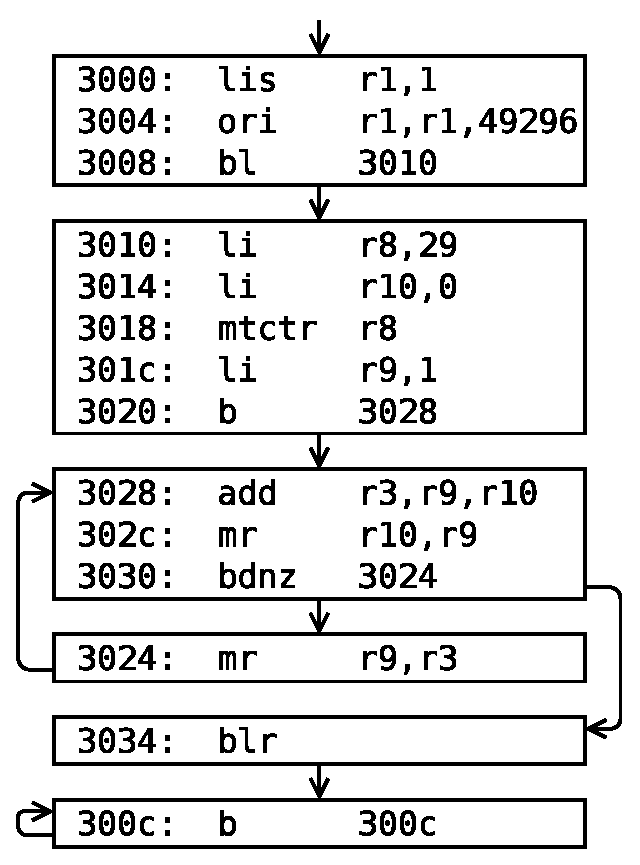
\includegraphics[scale=.4]{img/recons.eps}
        %\captionsetup{justification=centering}
        %\caption{CFG de \texttt{fibcall-O2.elf}}
        %\label{fig:recons}
      %\end{subfigure}
      %\caption{Processus de reconstruction d'un CFG}
%    \end{figure}

    % Définition de CFG et bloc de base

    %Un programme $P$ peut être décomposé en blocs de base.
    %Un bloc de base est une séquence d'instructions qui n'a qu'un point
    %d'entrée, sa première instruction, et qu'un point de sortie, sa dernière
    %instruction.
    %Un bloc de base est maximal s'il n'est pas possible de lui ajouter une instruction.
    %L'instruction de sortie d'un bloc de base maximal est donc nécessairement une instruction de branchement.
    %Dans la suite, on ne s'intéresse qu'aux blocs maximaux.
    
    %Le CFG d'un programme est un graphe orienté dans lequel les noeuds
    %représentent les blocs de base et les transitions représentent les
    %branchements possibles entre les différents blocs de base lors d'une
    %exécution du programme. Formellement, c'est un tuple $G = (V, E, u, v)$, où
    %les noeuds $V$ correspondent aux blocs de bases, les transitions $E \subset
    %V \times V$ sont les chemins du flot de contrôle, $u \in V$ représente le
    %n{\oe}ud d'entrée et $v \in V$ le n{\oe}ud de sortie.

    %Afin de procéder à la reconstruction du CFG d'une tâche, il faut tout
    %d'abord calculer les blocs de base. Cela se fait en identifiant les points
    %d'entrée des blocs puis en accumulant séquentiellement les instructions
    %d'un point d'entrée au suivant. Les points d'entrée sont : le point
    %d'entrée du programme ; les cibles des branchements ; les instructions qui
    %suivent immédiatement une instruction de branchement ; la première
    %instruction du fichier exécutable.
    %Le bloc qui commence au point d'entrée du programme est le n{\oe}ud initial du CFG.

    %Il faut ensuite en retrouver les transitions. Elles sont obtenues
    %itérativement en associant à chaque bloc de base les cibles possibles de
    %son point de sortie. Déterminer les cibles possibles d'un bloc de base
    %n'est pas une opération triviale, cela s'avère même parfois indécidable
    %statiquement dans le cas des branchements calculés résultant de la
    %compilation d'une structure de type \texttt{switch case} ou de la
    %manipulation de tableaux de pointeurs de fonctions.  Dans l'état actuel de
    %notre outil, l'utilisateur doit préciser les cibles des branchements
    %calculés.

    %La figure \ref{fig:dump} donne le code désassemblé du fichier binaire
    %exécutable \texttt{fibcall-O2.elf}.  La figure \ref{fig:recons} donne le
    %CFG reconstruit par notre outil à partir du fichier binaire exécutable
    %\texttt{fibcall-O2.elf}.


